%% Adaptado a partir de :
%%    abtex2-modelo-trabalho-academico.tex, v-1.9.2 laurocesar
%% para ser um modelo para os trabalhos no IFSP-SPO

\documentclass[
    % -- opções da classe memoir --
    12pt,               % tamanho da fonte
    openright,          % capítulos começam em pág ímpar (insere página vazia caso preciso)
    twoside,            % para impressão em verso e anverso. Oposto a oneside
    %oneside,
    a4paper,            % tamanho do papel. 
    % -- opções da classe abntex2 --
    %chapter=TITLE,     % títulos de capítulos convertidos em letras maiúsculas
    %section=TITLE,     % títulos de seções convertidos em letras maiúsculas
    %subsection=TITLE,  % títulos de subseções convertidos em letras maiúsculas
    %subsubsection=TITLE,% títulos de subsubseções convertidos em letras maiúsculas
    % Opções que não devem ser utilizadas na versão final do documento
    openany             %capitulos podem começar em página pares também
    draft,              % para compilar mais rápido, remover na versão final
    MODELO,             % indica que é um documento modelo então precisa dos geradores de texto
    TODO,               % indica que deve apresentar lista de pendencias 
    % -- opções do pacote babel --
    english,            % idioma adicional para hifenização
    brazil              % o último idioma é o principal do documento
    ]{ifsp-spo-inf-ctds}

        
% ---

% --- 
% CONFIGURAÇÕES DE PACOTES
% --- 
%\usepackage{etoolbox}
%\patchcmd{\thebibliography}{\chapter*}{\section*}{}{}
\usepackage{amsmath}
\usepackage{blindtext}
\usepackage{graphicx}

% ---
% CAPA e FOLHA DE ROSTO
% ---
\titulo{GinQuest: Aplicativo para criação e gerenciamento de gincanas}

\renewcommand{\imprimirautor}{
\begin{tabular}{lr}
Jones Sabino Silva & SP1672576 \\
Murilo Vicente da Silva & SP1674706 \\
Renata Monteiro Gadelha & SP1666339 \\
Rodrigo Bressan de Souza & SP167031X \\
Victor Hiroshi Castro Kawamoto & SP1670425 \\
\end{tabular}
}

\tipotrabalho{Projeto da Disciplina de Prática e Gerenciamento de Projetos}

\disciplina{A6PGP - Prática e Gerenciamento de Projetos}

\preambulo{Prova de conceito do projeto para disciplina de Prática e Gerenciamento de Projetos}

\data{2019}

% Utilizar o Nome Completo, abntex tem orientador e coorientador
% então vão ser utilizados na definição de professor
\renewcommand{\orientadorname}{Professor:}
\orientador{José Braz de Araújo}
\renewcommand{\coorientadorname}{Professor:}
\coorientador{Ivan Francolin Martinez}

% ---

% Configurações de aparência do PDF final


% informações do PDF
\makeatletter
\hypersetup{
        %pagebackref=true,
        pdftitle={\@title}, 
        pdfauthor={\@author},
        pdfsubject={\imprimirpreambulo},
        pdfcreator={LaTeX with abnTeX2},
        pdfkeywords={abnt}{latex}{abntex}{abntex2}{trabalho acadêmico}, 
        colorlinks=true,            % false: boxed links; true: colored links
        linkcolor=blue,             % color of internal links
        citecolor=blue,             % color of links to bibliography
        filecolor=magenta,              % color of file links
        urlcolor=blue,
        bookmarksdepth=4
}
\makeatother 
% --- 

% ---

% ----
% Início do documento
% ----
\begin{document}

% Retira espaço extra obsoleto entre as frases.
\frenchspacing 

\pretextual

% ---
% Capa - Para proposta a folha de rosto é suficiente pois é mais completa.
% ---
\imprimirfolhaderosto
% ---

% ----------------------------------------------------------
% ELEMENTOS TEXTUAIS
% ----------------------------------------------------------
\textual

{\let\clearpage\relax\par \chapter{Prova de Conceito}}

Este documento apresenta os requisitos exigidos para a prova de conceito da disciplina Práticas de Gerenciamento de Projetos comprovando a aderência das atividades desenvolvidas pela equipe GinQuest, identificando as tecnologias utilizadas no seu desenvolvimento e apresentando sua arquitetura.

Também foi solicitado gerar um vídeo utilizando a ferramenta Gource, no qual transforma o log de registro do repositório em uma árvore animada. Segundo a página institucional do \citeonline{gource}, o diretório raiz é localizado ao centro, os diretórios aparecem em forma de galhos e os arquivos aparecem como folhas. Os desenvolvedores são visualizados ao longo da árvore de acordo com as suas contribuições para o projeto.

Para uma visualização mais amigável foram realizados ajustes como a exibição do nome dos usuários e uma respectiva foto. Na Figura ~\ref{fig:gource} é possível ver um quadro do vídeo gerado.

Como comprovação da aderência da arquitetura foi solicitado um vídeo demonstrando a utilização do aplicativo, onde seja possível realizar um cadastro e bem como visualizar que os dados foram armazenados no banco de dados. O link da demonstração se encontra na seção de "Links da Prova de Conceito".

\begin{figure}
\caption{Vídeo gerado pela ferramenta Gource do projeto Ginquest}
\begin{center}
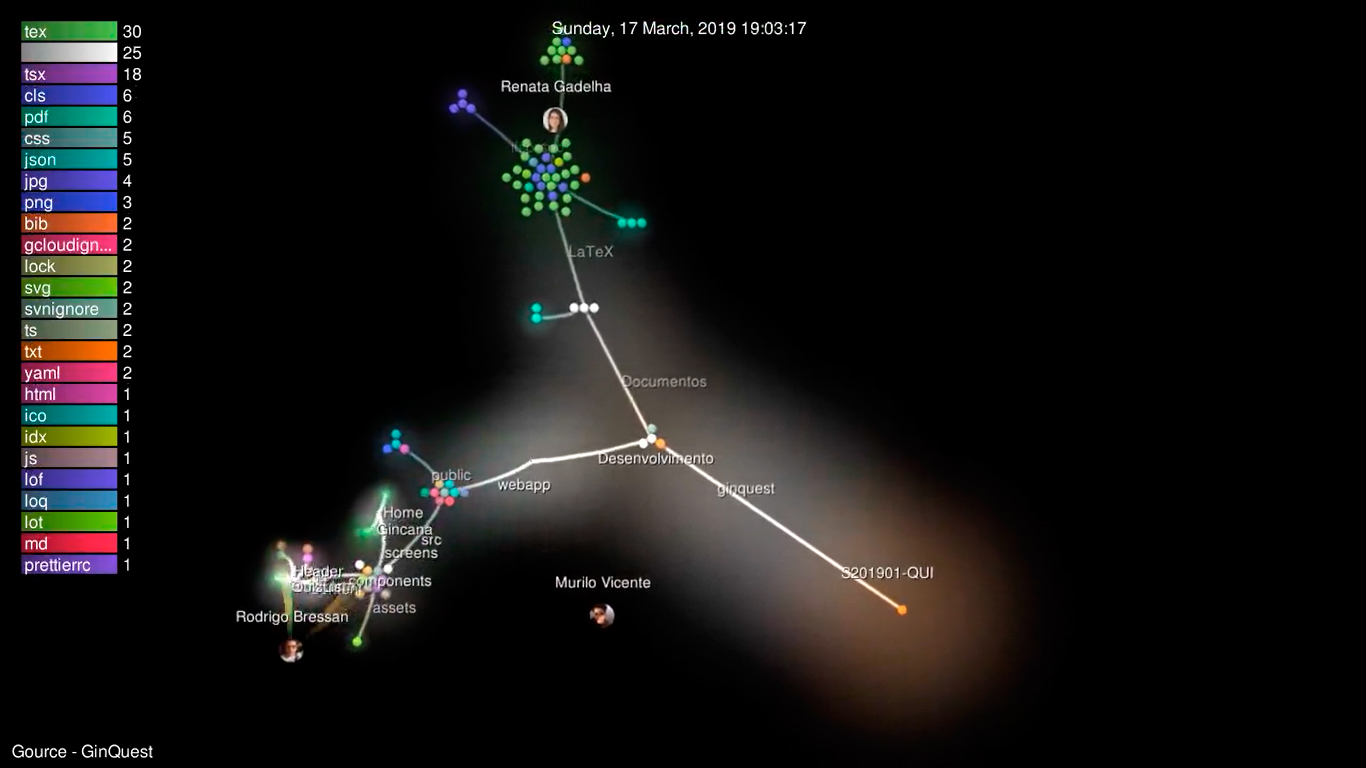
\includegraphics[scale=0.15]{images/poc/poc_gource.jpg}
\end{center}
\fonte{Autores do projeto}
\label{fig:gource}
\end{figure}

\vspace{1cm}
%{\let\clearpage\relax\par \chapter{Infraestutura}}
\section{Infraestutura}

A aplicação se encontra hospedada na plataforma Google Cloud Platform (GCP), uma suíte de computação em nuvem oferecida pelo Google. Da infraestrutura disponibilizada foi utilizado:


\begin{itemize}

\item 2 instâncias Google App Engine (GAE): plataforma como serviço (PaaS — Platform as a Service), em que é possível criar aplicações para a web, aplicativos móveis e até mesmo APIs, com a vantagem do dimensionamento automático. Esse recurso dimensiona as suas aplicações instantaneamente sempre que for preciso, de acordo com o tráfego que elas recebem. \cite{jackson2018}

\item Google Cloud Sql: Serviço de banco de dados relacionais MySQL e PostgreSQL na nuvem, que oferece altos níveis de desempenho e escalonabilidade. Para o projeto GinQuest, o PostgreSQL foi o escolhido.
\end{itemize}

%{\let\clearpage\relax\par \chapter{Arquitetura}}
\section{Arquitetura}

O Front-End (WebSite), o Back-End (API) e o banco de dados do projeto foram hospedados na plataforma Google Cloud Platform (GCP). A Figura  ~\ref{fig:arquitetura} mostra o modelo de arquitetura escolhido, onde o WebSite está disponível para os usuários em uma das instâncias do Google App Engine, a API está disponível para o WebSite na outra instância do Google App Engine e o banco de dados está disponível no Google Cloud SQL de modo a poder ser acessado pela API.

\begin{figure}
\caption{Diagrama de arquitetura do sistema GinQuest}
\begin{center}
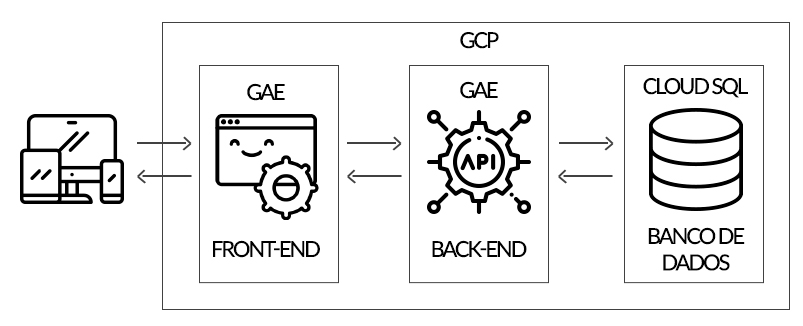
\includegraphics[scale=0.5]{images/poc/poc_arquitetura.jpg}
\end{center}
\fonte{Autores do projeto}
\label{fig:arquitetura}
\end{figure}

%{\let\clearpage\relax\par \chapter{Tecnologias Utilizadas}}

As tecnologias utilizadas no Front-end, além do uso de HTML5 como linguagem de marcação e CSS3 para estilo das páginas, o framework Bootstrap e React, de maneira a se tornar uma aplicação Web responsiva, seguindo o conceito "mobile-first". No back-end foi utilizado Javascript com o framework Express para gerenciar as requisições e respostas HTTP, de modo a criar uma API no modelo REST, que terá acesso ao banco de dados relacional PostgreSQL.

\begin{itemize}

\item Bootstrap: framework web para desenvolvimento de componentes de interface e front-end para sites e aplicações web usando HTML, CSS e JavaScript. Ele permite a criação com responsividade e "mobile-first", isto é, com foco em dispositivos móveis \cite{bootstrap}. 
\item React: biblioteca JavaScript para criação de interfaces de usuário.
\item Express: framework para aplicativo da web do Node.js mínimo e flexível que fornece um conjunto robusto de recursos para aplicativos web e móvel. \cite{express}.
\item PostgreSQL: sistema gerenciador de banco de dados objeto relacional.
\end{itemize}

%\vspace{1cm}
%{\let\clearpage\relax\par \chapter{Links da Prova de Conceito}}
\section {Links da Prova de Conceito}

\begin{itemize}
\item Aplicação GinQuest: https://ginquest-app.appspot.com
\item Vídeo Gource: https://www.youtube.com/watch?v=I2WxAHn-NGo
\item Vídeo de demonstração da aplicação: https://www.youtube.com/watch?v=KrOlskd2Xno
\end{itemize}


% ----------------------------------------------------------
% Referências bibliográficas
% ----------------------------------------------------------
\bibliography{referencias,exemplos/abntex2-doc-abnt-6023}

\end{document}